Embarking on the findings of this chapter, I transition from the established COMSOL modeling workflow to the critical stage of validating theoretical concepts through the lens of computational analysis. The essence of this chapter is twofold: first, to harness the computational prowess of COMSOL in validating key optical phenomena such as anti-reflectivity thus corroborate our simulation outcomes with theoretical models; and second, to attempt to model the simplest Passive Daytime Radiative Cooling devices (PDRCs) at Hudgings Lab by showing how their reflectance varies with wavelength.

My investigation begins with an empirical analysis of anti-reflective behaviors, examining both simple and composite multilayer arrangements. These simulations are meticulously compared to the theoretical predictions presented in \emph{Introduction to Optics} by Frank L. Pedrotti et al. \cite{pedrotti_introduction_2007}.

It is crucial to acknowledge—as delineated in Chapter 2—the analytical derivation of reflectance as a function of angle $R(\theta)$ and wavelength $R(\lambda)$ is straightforward for materials with a constant refractive index $n$. However, the complexity escalates when dealing with materials where the refractive index varies with $\lambda$, a common occurrence in real-world applications. This variation poses significant challenges to traditional analytical methods, thereby necessitating the adoption of sophisticated computational tools like COMSOL for accurate simulations.

We delve into the intricacies of high reflectance by simulating stacks of alternating high and low refractive index layers, shedding light on the nuanced ways layer configurations impact reflectance. These insights are bench-marked against scholarly literature, reinforcing the accuracy of our models.

Moreover, the thesis explores the layered design of PDRCs. By systematically layering silicon, silver, and Polydimethylsiloxane (PDMS), we dissect the optical properties crucial to the development of passive cooling systems. The collection of results and graphs here encapsulate more than just data; they are catalysts for continuous inquiry and deeper understanding of optical physics as it related to PDRCs.

% ---------- SECTION: COMSOL: MODELING ANTI-REFLECTANCE COATINGS ----------

\section{COMSOL: Modeling Anti-Reflectance Coatings}

As we progress in our exploration of anti-reflectance coatings, it is beneficial to revisit the foundational principles that govern their behavior. These coatings are designed to minimize reflection and maximize transmission of light through strategic manipulation of refractive indices across different layers.

To appreciate the mathematical underpinnings of these designs, recall a pivotal formula, Equation \ref{reflectance for 2-layer antireflecting films}, that encapsulates the essence of a two-layer anti-reflecting film's performance. Assuming light strikes normally on the film, the reflectance, $R$, can be described by the following relationship:

\begin{equation}\label{reflectance for 2-layer antireflecting films - chap4}
    R = \left(\frac{n_0n_2^2 - n_sn_1^2}{n_0n_2^2 + n_sn_1^2}\right)^2
\end{equation}

Here, we anticipate zero reflectance when the expression in the numerator becomes zero, leading us to equation \ref{zero reflectance criterion}, which stipulates the condition for achieving no reflectance:

\begin{equation}\label{zero reflectance criterion - chap4}
    \frac{n_2}{n_1} = \sqrt{\frac{n_s}{n_0}}
\end{equation}

This relationship delineates the necessary ratio between the refractive indices of the layers that leads to a reflectance of zero.

When working with a glass substrate of refractive index $n_s = 1.5$ and air of refractive index $n_0 = 1$, the ideal refractive index ratio, $\frac{n_2}{n_1}$, is calculated to be $\sqrt{1.5} \approx 1.225$.

In COMSOL, our goal is to identify and define (in our parameters table) two materials for the double-layer structure that closely match this ratio to maximize anti-reflective properties. It is crucial to note that the refractive index of most materials varies with wavelength. This variability, known as dispersion, means that optimal thickness and refractive indices for minimizing reflectance at one wavelength may not be as effective at another. While it is challenging to select materials that precisely align their refractive indices to achieve exactly zero reflectance, our aim is to get as close to 0\% reflectance over as wide a $\lambda$ range as practically possible.

The limitation of a quarter-wavelength layer is its selective reflectivity; it effectively eliminates reflection at a specific wavelength but substantially reflects at other wavelengths in proximity. Additionally, its performance varies significantly with the angle at which light strikes the surface. A viable solution to overcome this is the application of multilayer coatings. These coatings, compared to their single-layer counterparts, tend to lower the reflection coefficient over a broader spectrum and accommodate a greater diversity of tangible materials \cite{pedrotti_introduction_2007}.

In the following section, we will compare the reflectivity of two distinct multilayer coatings across an extensive spectral range. The analysis will cover a dual-layer (quarter-quarter wavelength coating) and a triple-layer (quarter-half-quarter wavelength coating). It will be demonstrated that the triple-layer coating achieves a more uniform low reflectance throughout the majority of the visible light spectrum.

% ---------- SUBSECTION: ANTI-REFLECTANCE LAYERS: SETUP ----------

\subsection{Anti-reflectance Layers: Setup}

The pursuit of anti-reflective coatings leads us to the utilization of thin film dielectrics within COMSOL. In line with the criteria for zero reflectance, the first dielectric film, starting from the base, is cerium trifluoride ($\text{CeF}_3$) with a refractive index of 1.63, while the second film is magnesium fluoride ($\text{MgF}_2$) with a refractive index of 1.38. The refractive index ratio of approximately 1.181 aligns closely with the optimal ratio of 1.225. As established in chapter 2, effective anti-reflectivity for a dual-layer arrangement requires each film to be a quarter-wavelength in thickness, which corresponds to the wavelength at which minimal reflectance is desired.

\begin{figure}[H]
  \centering
  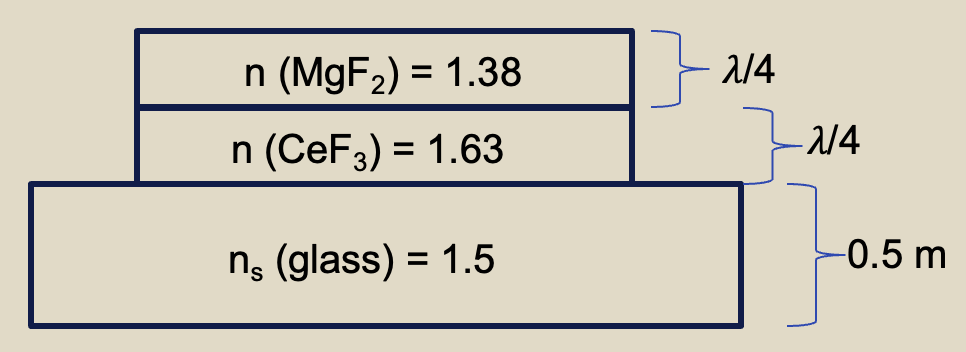
\includegraphics[width=0.7\textwidth]{Chapters/Figures/Chapter 4 Figures/Antireflective Double-Layer (PowerPoint).png}
  \caption{The double-layer anti-reflectance coating layout (dimensions not to scale). Source: created by the author using Microsoft PowerPoint.}
  \label{fig:Antireflective Double-Layer (PowerPoint)}
\end{figure}

In our enhanced three-layer structure, designed to broaden anti-reflectivity across a larger wavelength spectrum, the middle layer is a half-wavelength film of zirconium dioxide ($\text{ZrO}_2$), chosen for its refractive index of 2.2. This multi-layer configuration allows for increased anti-reflective performance compared to the more wavelength-specific two-layer model.

\begin{figure}[H]
  \centering
  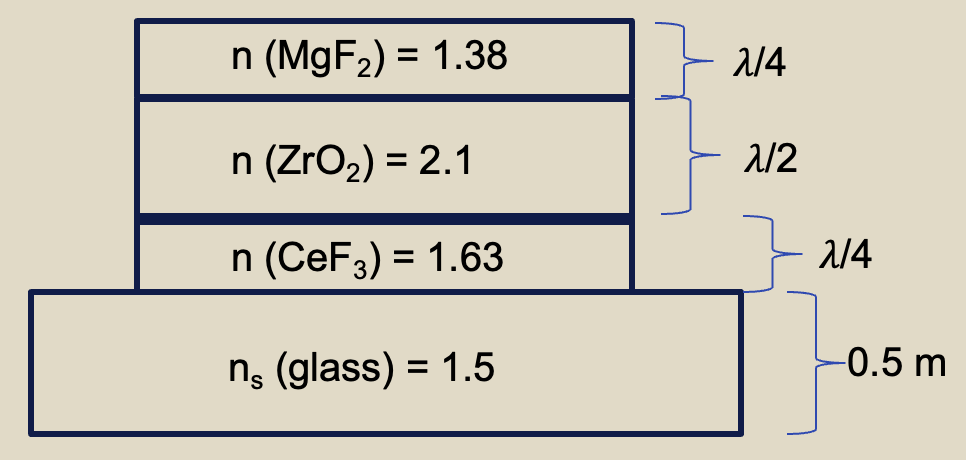
\includegraphics[width=0.7\textwidth]{Chapters/Figures/Chapter 4 Figures/Antireflective Triple-Layer (PowerPoint).png}
  \caption{The triple-layer anti-reflectance coating layout (dimensions not to scale). Source: created by the author using Microsoft PowerPoint.}
  \label{fig:Antireflective Triple-Layer (PowerPoint)}
\end{figure}

This screenshot from the COMSOL desktop highlights the configuration for modeling anti-reflective coatings. Pay particular attention to the 'Film Properties' area within the 'Thin Dielectric Film' settings where the quarter-wavelength calculation is outlined.

\begin{figure}[H]
  \centering
  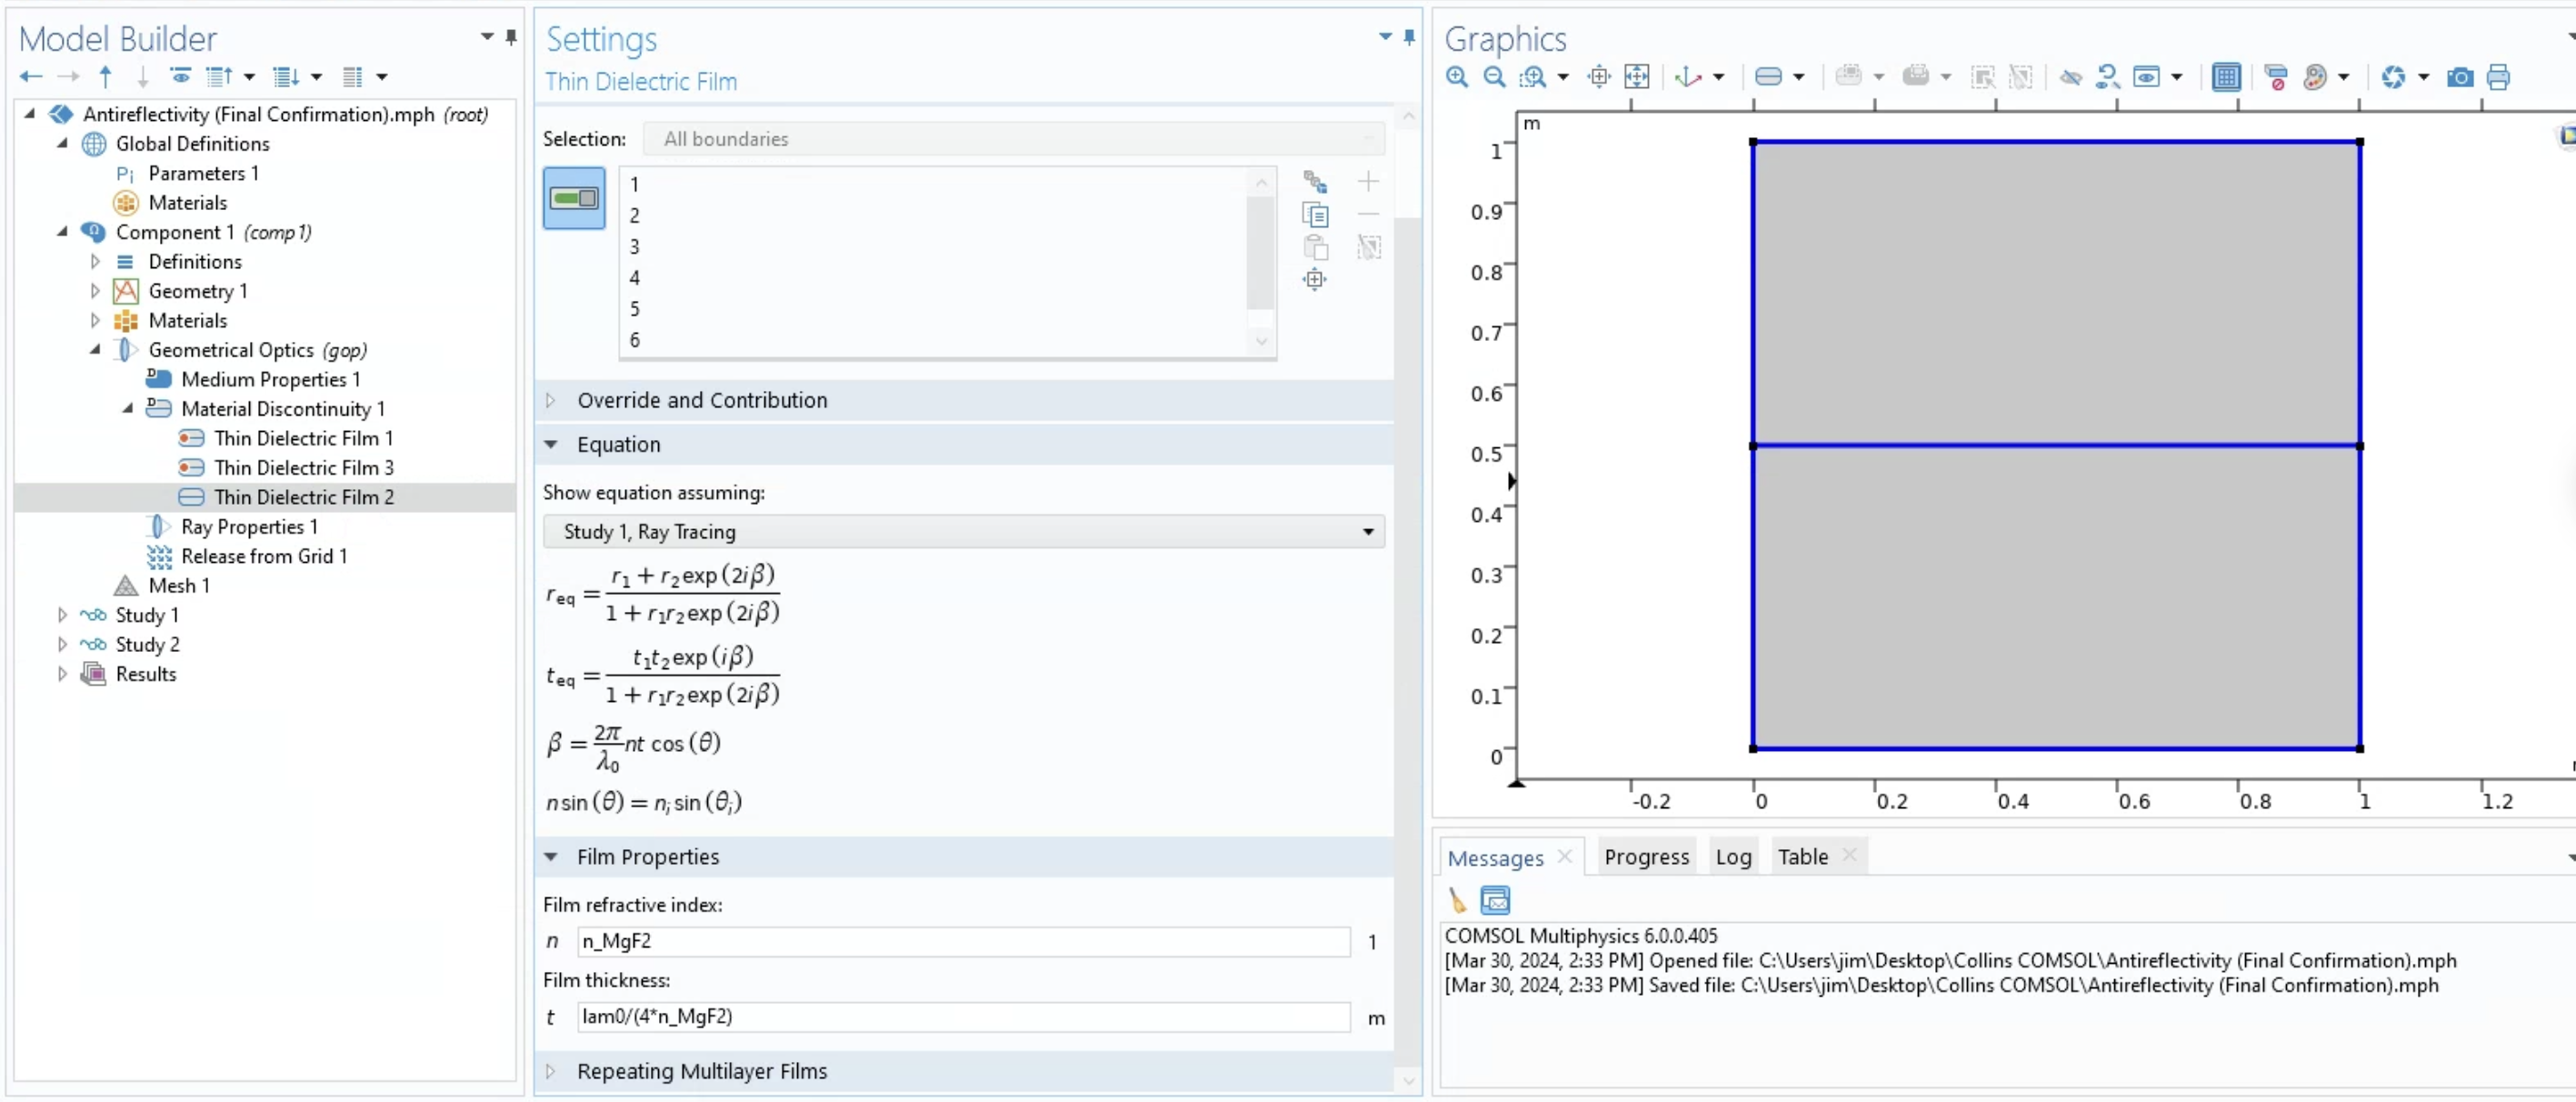
\includegraphics[width=0.7\textwidth]{Chapters/Figures/Chapter 4 Figures/COMSOL Desktop Showcasing Antireflectivity Setup.png}
  \caption{COMSOL desktop setup showcasing anti-reflectivity modeling.}
  \label{fig:COMSOL desktop showcasing antireflectivity}
\end{figure}

Here, the findings from the anti-reflectivity modeling using $\text{CeF}_3$ and $\text{MgF}_2$ for the quarter-quarter wavelength combination, as well as $\text{CeF}_3$, $\text{MgF}_2$, and $\text{ZrO}_2$ for the quarter-half-quarter wavelength setup, are presented.

\begin{figure}[H]
  \centering
  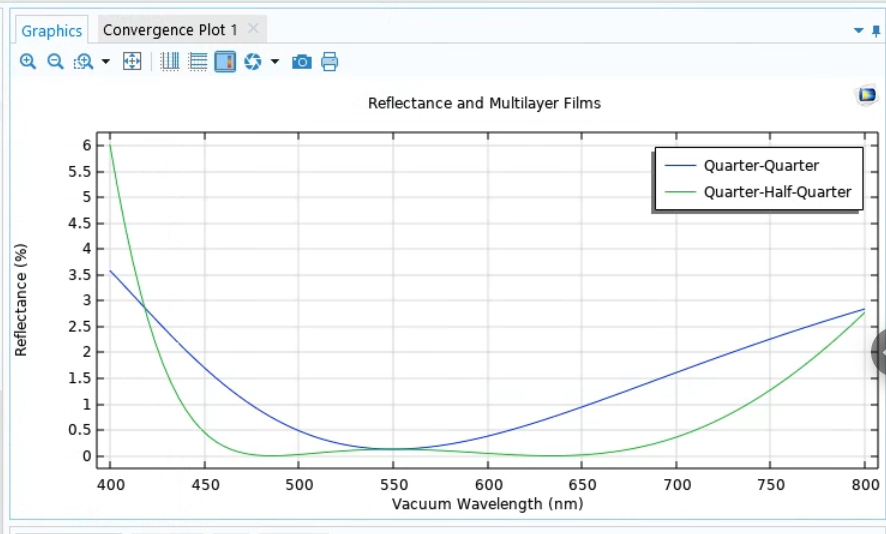
\includegraphics[width=0.7\textwidth]{Chapters/Figures/Chapter 4 Figures/Quarter-Half-Quarter.png}
  \caption{Illustration of the reflectance behavior for two anti-reflective coating configurations across the visible light spectrum. The blue line indicates the performance of a quarter-quarter wavelength coating, whereas the green line shows the effect of a quarter-half-quarter wavelength coating.}
  \label{fig:both quarter-quarter and quarter-half-quarter}
\end{figure}

In the quarter-quarter wavelength design, we employ two layers, each precisely a quarter of the desired wavelength in thickness. While the aim is to achieve minimal reflectance at a particular wavelength, the actual reflectance seldom reaches absolute zero due to the inherent limitations of material characteristics.

On the other hand, the quarter-half-quarter arrangement introduces an additional layer, half a wavelength thick, nestled between two quarter-wavelength films. This configuration is tailored to minimize reflectance across an extended spectrum of wavelengths.

Such multi-layered coatings surpass the effectiveness of single-layer films for anti-reflective purposes by accommodating a wider wavelength range. This versatility is particularly beneficial in applications where reducing reflection is paramount, such as in the manufacturing of optical lenses.

% ---------- SUBSECTION: VERIFYING ANTI-REFLECTANCE COMPUTATIONAL RESULTS THROUGH COMPARISON WITH THEORETICAL OPTICS LITERATURE ----------

\subsection{Verifying Anti-Reflectance Computational Results Through Comparison with Theoretical Optics Literature}

This section aims to validate the obtained computational results with the principles outlined in \emph{Introduction to Optics} by Frank L. Pedrotti et al \cite{pedrotti_introduction_2007}.

Beginning with a straightforward approach, we examine the reflectance across various wavelengths for three distinct multilayer film configurations:
\begin{enumerate}
    \item Films with quarter-quarter wavelength thickness.
    \item Films with quarter-half wavelength thickness.
    \item Films with quarter-half wavelength thickness, incorporating a different material for the half-wavelength layer.
\end{enumerate}

\begin{figure}[H]
  \centering
  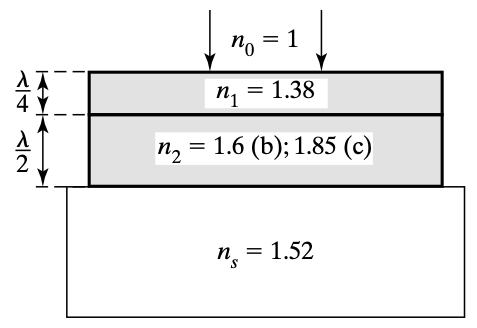
\includegraphics[width=0.7\textwidth]{Chapters/Figures/Chapter 4 Figures/Antireflecting Double Layer using Quarter and Half-Wavelength Thickness Films Layout.png}
  \caption{Antireflective double-layer arrangement. Source: \cite{pedrotti_introduction_2007}}
  \label{fig:antireflective_double_layer}
\end{figure}

We first examine films with quarter-quarter wavelength thickness. The reference from Pedrotti et al. specifies the lower thin dielectric layer as $\text{ZrO}_2$ and places $\text{CeF}_3$ directly above. The choice of materials is flexible, provided they adhere to the optimal ratio criterion for anti reflectance as defined in equation \ref{zero reflectance criterion - chap4}. This results in a refractive index ratio of $\frac{n_2}{n_1} = \frac{2.1}{1.65} \approx 1.273$, aligning closely with the ideal ratio of approximately 1.225 for normal incidence, given a substrate refractive index ($n_s$) of 1.5.

Expanding the spectrum of low reflectance within the visible region becomes achievable by diverging from the constraint of equal quarter-wavelength ($\lambda/4$) coatings. By integrating a layer of quarter-wavelength thickness as the second layer (considered from the bottom upwards), we attain more extensive zones of diminished reflectance. Consequently, in the scenario of item 2, we employ magnesium fluoride ($\text{MgF}_2$), characterized by a refractive index of 1.38, as the quarter-wavelength thick material. The intermediate half-wavelength layer utilizes aluminum oxide, with a refractive index of 1.60. For item 3, thorium dioxide, featuring a refractive index of 1.85, serves as the material for the half-wavelength thick layer, as noted in \cite{pedrotti_introduction_2007}.

For the specific wavelength of 550 nm, where the thicknesses of the quarter-wavelength ($\lambda/4$) and half-wavelength ($\lambda/2$) layers are calculated, the half-wavelength layer does not influence reflectance. In this case, the double-layer system acts akin to a solitary quarter-wavelength layer, resulting in a reflectance of 1.3\%. At wavelengths close to 550 nm, the presence of the half-wavelength layer contributes to maintaining reflectance levels below those achieved by a two quarter-wavelength layers. Below is the plot illustrating reflectance against wavelength for scenarios 1 through 3.

The graph below illustrates anti-reflectivity trends as detailed in the Optics textbook, indicating that while the reflectance at a wavelength of 550 nm stands at approximately 1.3\%, this value surpasses the performance of the quarter-quarter wavelength coating. Nevertheless, reflectance stays below this threshold across a wide wavelength span, extending from roughly 420 to 800 nm. This suggests that alternative configurations for dual-layer reflective films could be viable if the layers are not strictly constrained to quarter-wavelength multiples.

\begin{figure}[H]
  \centering
  % Top left figure
  \begin{minipage}{0.45\textwidth}
    \centering
    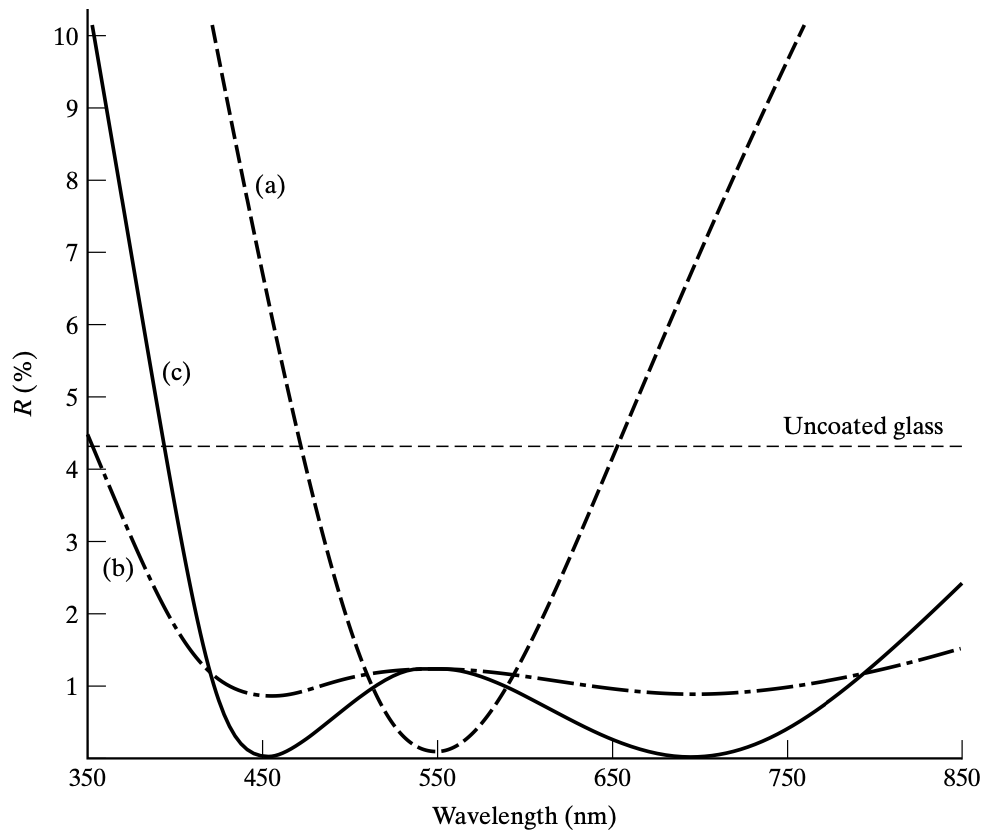
\includegraphics[width=\textwidth]{Chapters/Figures/Chapter 4 Figures/Antireflectivity Graphs in the Optics Book.png}
    \caption{Anti-reflectivity Graphs as shown in the Optics Textbook.}
    \label{fig:antireflectivity graphs in the Optics book}
  \end{minipage}\hfill
  % Top right figure
  \begin{minipage}{0.45\textwidth}
    \centering
    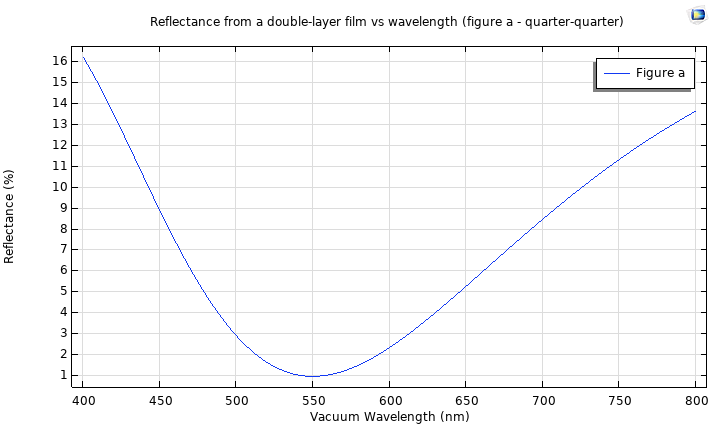
\includegraphics[width=\textwidth]{Chapters/Figures/Chapter 4 Figures/Anti-Reflectance Figure a.png}
    \caption{Modeling results of an anti-reflective coating with two layers, each a quarter-wavelength thick.}
    \label{fig:Antireflective Figure a}
  \end{minipage}
  % Bottom left figure
  \begin{minipage}{0.45\textwidth}
    \centering
    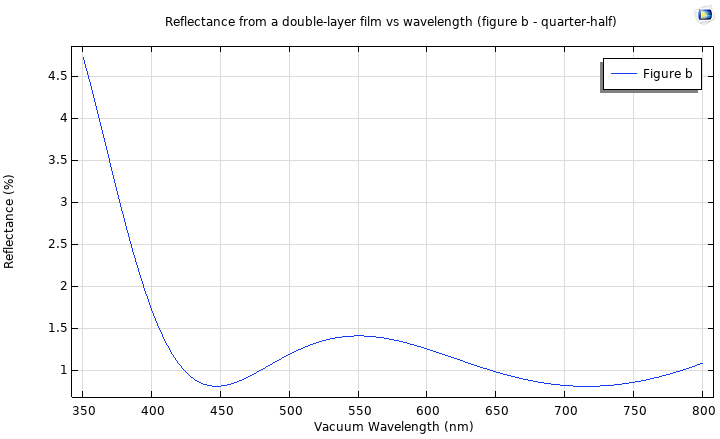
\includegraphics[width=\textwidth]{Chapters/Figures/Chapter 4 Figures/Anti-Reflectance Figure b.png}
    \caption{Reflectance outcomes for an anti-reflective coating with a bottom layer a quarter-wavelength thick and a top layer half-wavelength thick, using a material with a refractive index of 1.6.}
    \label{fig:Antireflective Figure b}
  \end{minipage}\hfill
  % Bottom right figure
  \begin{minipage}{0.45\textwidth}
    \centering
    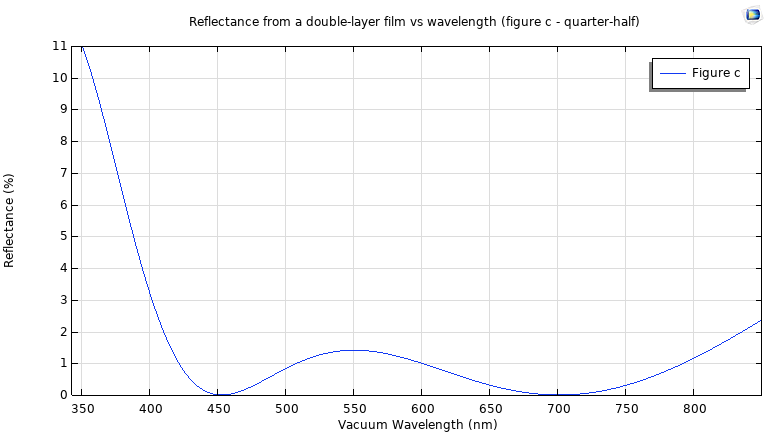
\includegraphics[width=\textwidth]{Chapters/Figures/Chapter 4 Figures/Anti-Reflectance Figure c.png}
    \caption{Reflectance results for an anti-reflective double layer with a bottom layer a quarter-wavelength thick and a top layer half-wavelength thick, using a material with a refractive index of 1.85.}
    \label{fig:Antireflective Figure c}
  \end{minipage}
\end{figure}

These results derive from the principles outlined in Chapter 2. Initially, the overall transfer matrix elements are calculated by multiplying the transfer matrices of the individual layers together. Within these calculations, the phase difference, $\delta$, varies with $\lambda$, aligning the film thickness with either $\lambda/4$ or $\lambda/2$ at the reference wavelength of 550 nm.

Subsequently, the reflection coefficient, as outlined in \ref{reflection coefficient in terms of transfer matrix terms}, is squared to produce reflectance as a wavelength function. COMSOL's Ray Optics module significantly simplifies this process by automating several steps, although careful consideration is needed for layer treatment, particularly regarding their classification as thin dielectric films.

\section{COMSOL: Modeling High Reflectance.}
To achieve anti-reflective properties, layers are arranged starting from the air and progressing through low-index to high-index materials before reaching the substrate. In contrast, for enhanced reflectivity, the sequence is reversed, starting from the air to high-index and then to low-index materials before ending at the substrate. This arrangement encourages multiple reflections of the incident light within the layered structure.

A combination of layers arranged to maximize reflectivity is known as a \emph{dielectric mirror}, \emph{high-reflectance stack}, or \emph{distributed Bragg reflector}. It's important to note that achieving high reflectance across the solar spectrum is a key factor for effective passive daytime radiative cooling, as previously discussed.

\begin{figure}[H]
  \centering
  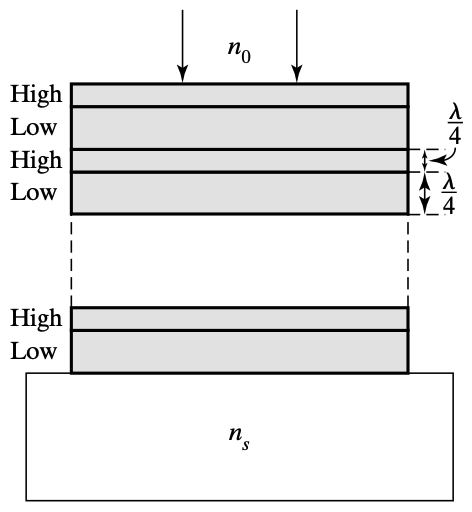
\includegraphics[width=0.5\textwidth]{Chapters/Figures/Chapter 4 Figures/High-Reflectance Stack of Double Layers.png}
  \caption{High-reflectance stack comprising double layers with alternating high and low refractive indices. Source: \cite{pedrotti_introduction_2007}}
  \label{fig:visualizing high-reflectance stack with alternating indices}
\end{figure}

% ---------- SUBSECTION: VERIFYING HIGH REFLECTANCE COMPUTATIONAL RESULTS THROUGH COMPARISON WITH THEORETICAL OPTICS LITERATURE ----------

\subsection{Verifying High Reflectance Computational Results Through Comparison with Theoretical Optics Literature}
The formula to ascertain high reflectance, $R$, at a chosen design wavelength ($\lambda_0$) for a specific layer arrangement is denoted by \ref{maximum reflectance equation}.

\begin{equation}\label{formula for optimal reflectance - chap4}
    R = \left[ \frac{ \left( \frac{n_0}{n_s} \right) \left( \frac{n_L}{n_H} \right)^{2N}  - 1 }{  \left( \frac{n_0}{n_s} \right) \left( \frac{n_L}{n_H} \right)^{2N}  + 1}  \right]^2
\end{equation}

Achieving maximal reflectance (100\%) occurs under the following conditions:
\begin{enumerate}
    \item As $N$, representing the count of layer pairs, becomes very large.
    \item When the ratio $\frac{n_L}{n_H}$ approaches zero.
\end{enumerate}

The optics textbook illustrates high reflectance with the following depiction:

\begin{figure}[H]
  \centering
  % Left figure
  \begin{minipage}{0.48\textwidth}
    \centering
    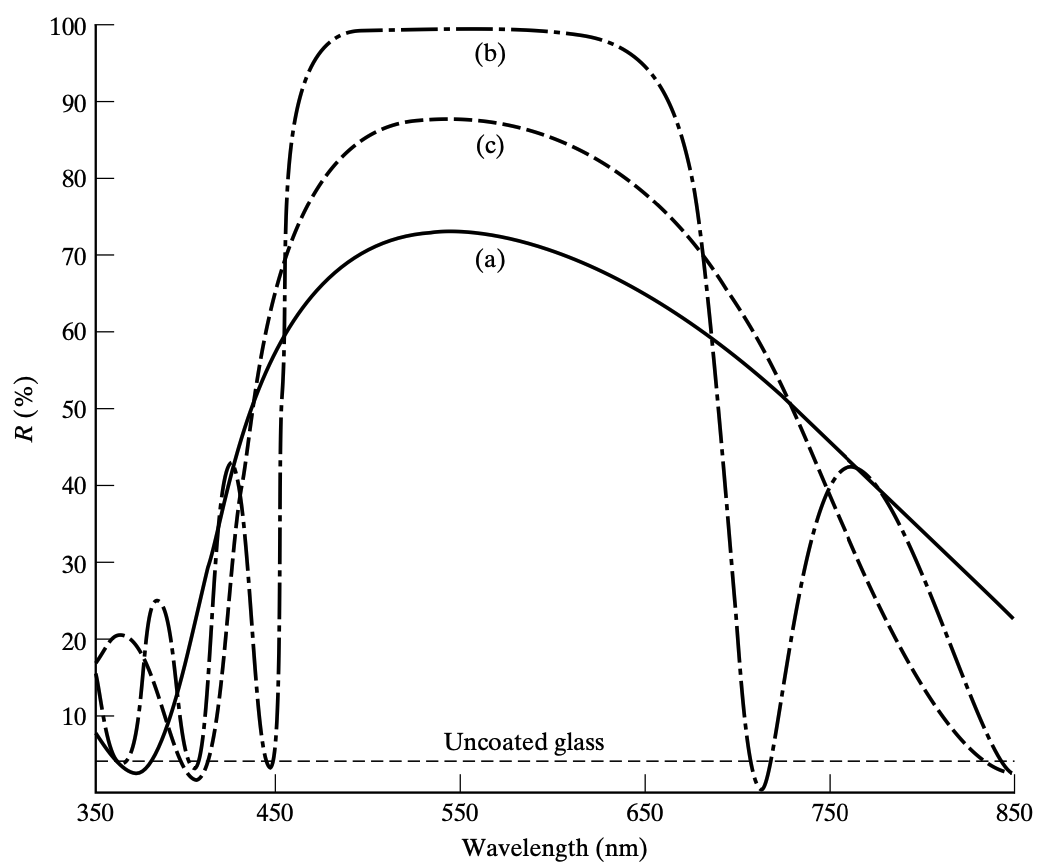
\includegraphics[width=\textwidth]{Chapters/Figures/Chapter 4 Figures/High-Reflectance Graphs in the Optics Book.png}
    \caption{Reflectance spectra for high-low index stacks: (a) for a two-layer double stack, (b) for a six-layer double stack, and (c) for a two-layer double stack enhanced with an additional high-index layer at the very top. Source: \cite{pedrotti_introduction_2007}}
    \label{fig:Reflectance spectra from optical literature}
  \end{minipage}\hfill
  % Right figure
  \begin{minipage}{0.48\textwidth}
    \centering
    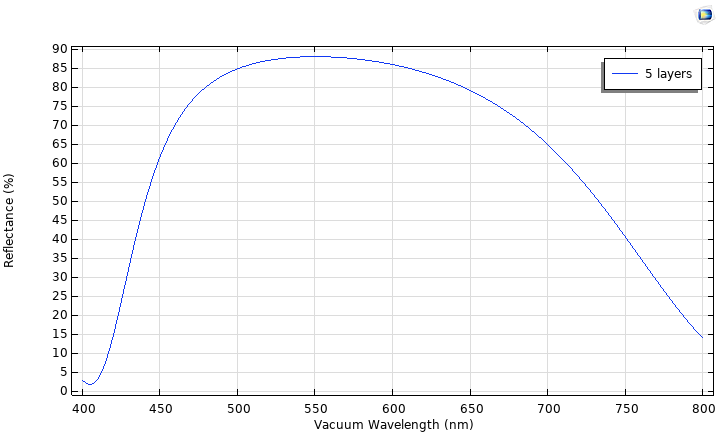
\includegraphics[width=\textwidth]{Chapters/Figures/Chapter 4 Figures/High-Reflectance (5 Layers).png}
    \caption{Spectral reflectance for a structure with two pairs of high-low refractive index layers, topped with an additional high-index layer. This figure is similar to plot (c) present in the left figure.}
    \label{fig:Reflectance 5-layer structure}
  \end{minipage}
\end{figure}

In these configurations, layers are designed to be $\lambda/4$ thick at a design wavelength $\lambda_0 = 550$ nm. Here, the high-index material (Zinc Sulfide - ZnS) has $n_H = 2.35$, the low-index material (Magnesium Fluoride - $\text{MgF}_2$) has $n_L = 1.38$, and the incident medium (air) has $n_0 = 1.00$. The ratio of $\frac{n_L}{n_H}$ is thus approximately $\frac{1.38}{2.35} \approx 0.587$.

Our analysis will specifically address graph (c), which demonstrates how adding an extra high-index layer between the substrate and the final low-index layer enhances maximum reflectance in a two-layer double stack ($N = 2$). This addition improves reflectance efficiency compared to simpler two-layer double configurations.

The findings showcased below stem from applying the high reflectance principles discussed in Chapter 2.

Observe the alignment of peak reflectance with the textbook's findings, achieving 90%.

Employing a parametric sweep in COMSOL allows for the exploration of reflectance variation across wavelengths by systematically adjusting the count of double layer pairs ($N$) to values such as 2, 5, 10, and 20. This approach calculates solutions across a range of parameter sets. For all depicted graphs, an extra top layer with a high refractive index is incorporated to broaden the spectrum of maximum reflectance.

\begin{figure}[H]
  \centering
  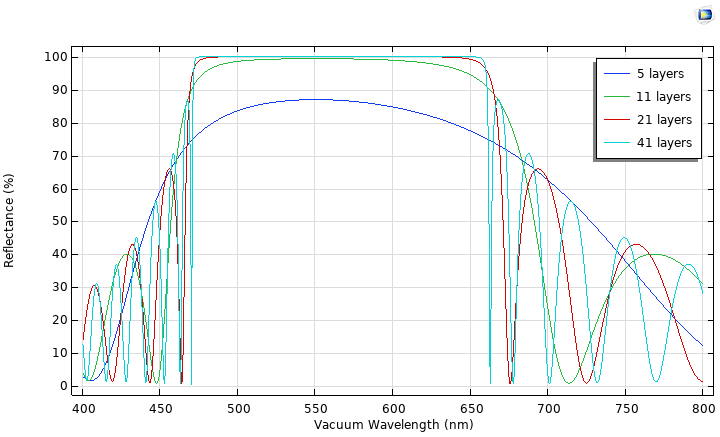
\includegraphics[width=0.7\textwidth]{Chapters/Figures/Chapter 4 Figures/High-Reflectance (5, 11, 21, and 41 Layers).png}
  \caption{Reflectance comparison for configurations with 5, 11, 21, and 41 layers, each enhanced by an additional high-index surface layer.}
  \label{fig:COMSOL multi-layer reflectance results}
\end{figure}

Unlike conventional metallic mirrors, DBRs leverage a careful and simple engineered structure of alternating thin layers of materials with contrasting refractive indices. This design typically features an odd number of layers, anchored by high refractive index materials at both ends, optimizing their reflectivity \cite{multiphysics__distributed_nodate}.

At the core of a DBR's functionality is the concept of constructive interference. As optical waves encounter the boundaries between layers, each boundary induces a partial reflection. When the optical wave's wavelength is four times the layers' optical thickness, these reflections interfere constructively, transforming the layers into an efficient reflector. This principle gives rise to a \emph{stopband}, a wavelength range where the reflector achieves heightened reflection. With an adequate number of layers, a DBR can achieve a high-quality reflection, making it useful in the operation of vertical cavity surface emitting lasers \cite{multiphysics__distributed_nodate}.

Expanding beyond the \emph{stopband}, DBRs exhibit a characteristic where reflectance transitions into a pattern of oscillating maxima and minima. By strategically adjusting these parameters, it is possible to shift the stopband's center, enhancing the filter's spectral transmittance across a broader range. This capability to finely control the light's passage through these structures not only underscores the versatility of DBRs but also paves the way for their integration into a wide array of optical devices, where precise manipulation of light is paramount \cite{pedrotti_introduction_2007}.

% ----- SECTION: COMSOL: MODELING PDRCs -----

\section{COMSOL: Modeling PDRCs}
At Hudgings Lab, one of the foundational PDRC designs comprises a straightforward sequence of layers. Beginning with silicon as the foundation, a layer of silver is applied directly above, topped with a final layer of Polydimethylsiloxane (PDMS).

\begin{figure}[H]
  \centering
  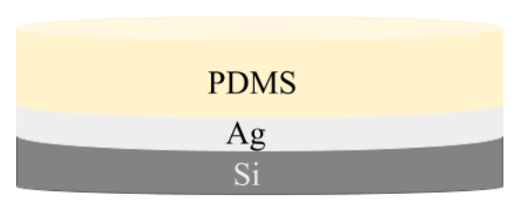
\includegraphics[width=0.7\textwidth]{Chapters/Figures/Chapter 4 Figures/PDRC Layout.png}
  \caption{Illustration of a basic PDRC configuration at Hudgings Lab, featuring a silicon base with subsequent layers of silver and PDMS.}
  \label{fig:PDRC-configuration-Hudgings-Lab}
\end{figure}

To understand the optical behavior of this structure, I systematically approached the modeling process from the bottom layer upwards. The following results present a sequence of reflectance versus wavelength analyses for each layer configuration: initially for silicon, followed by silicon with an added silver layer, and concluding with the composite structure of silicon, silver, and PDMS. This progression illustrates how each layer contributes to the overall reflectance spectrum.

% ----- SUBSECTION: ANALYSIS OF SILICON LAYER ONLY -----

\subsection{Analysis of Silicon Layer Only}

\begin{figure}[H]
  \centering
  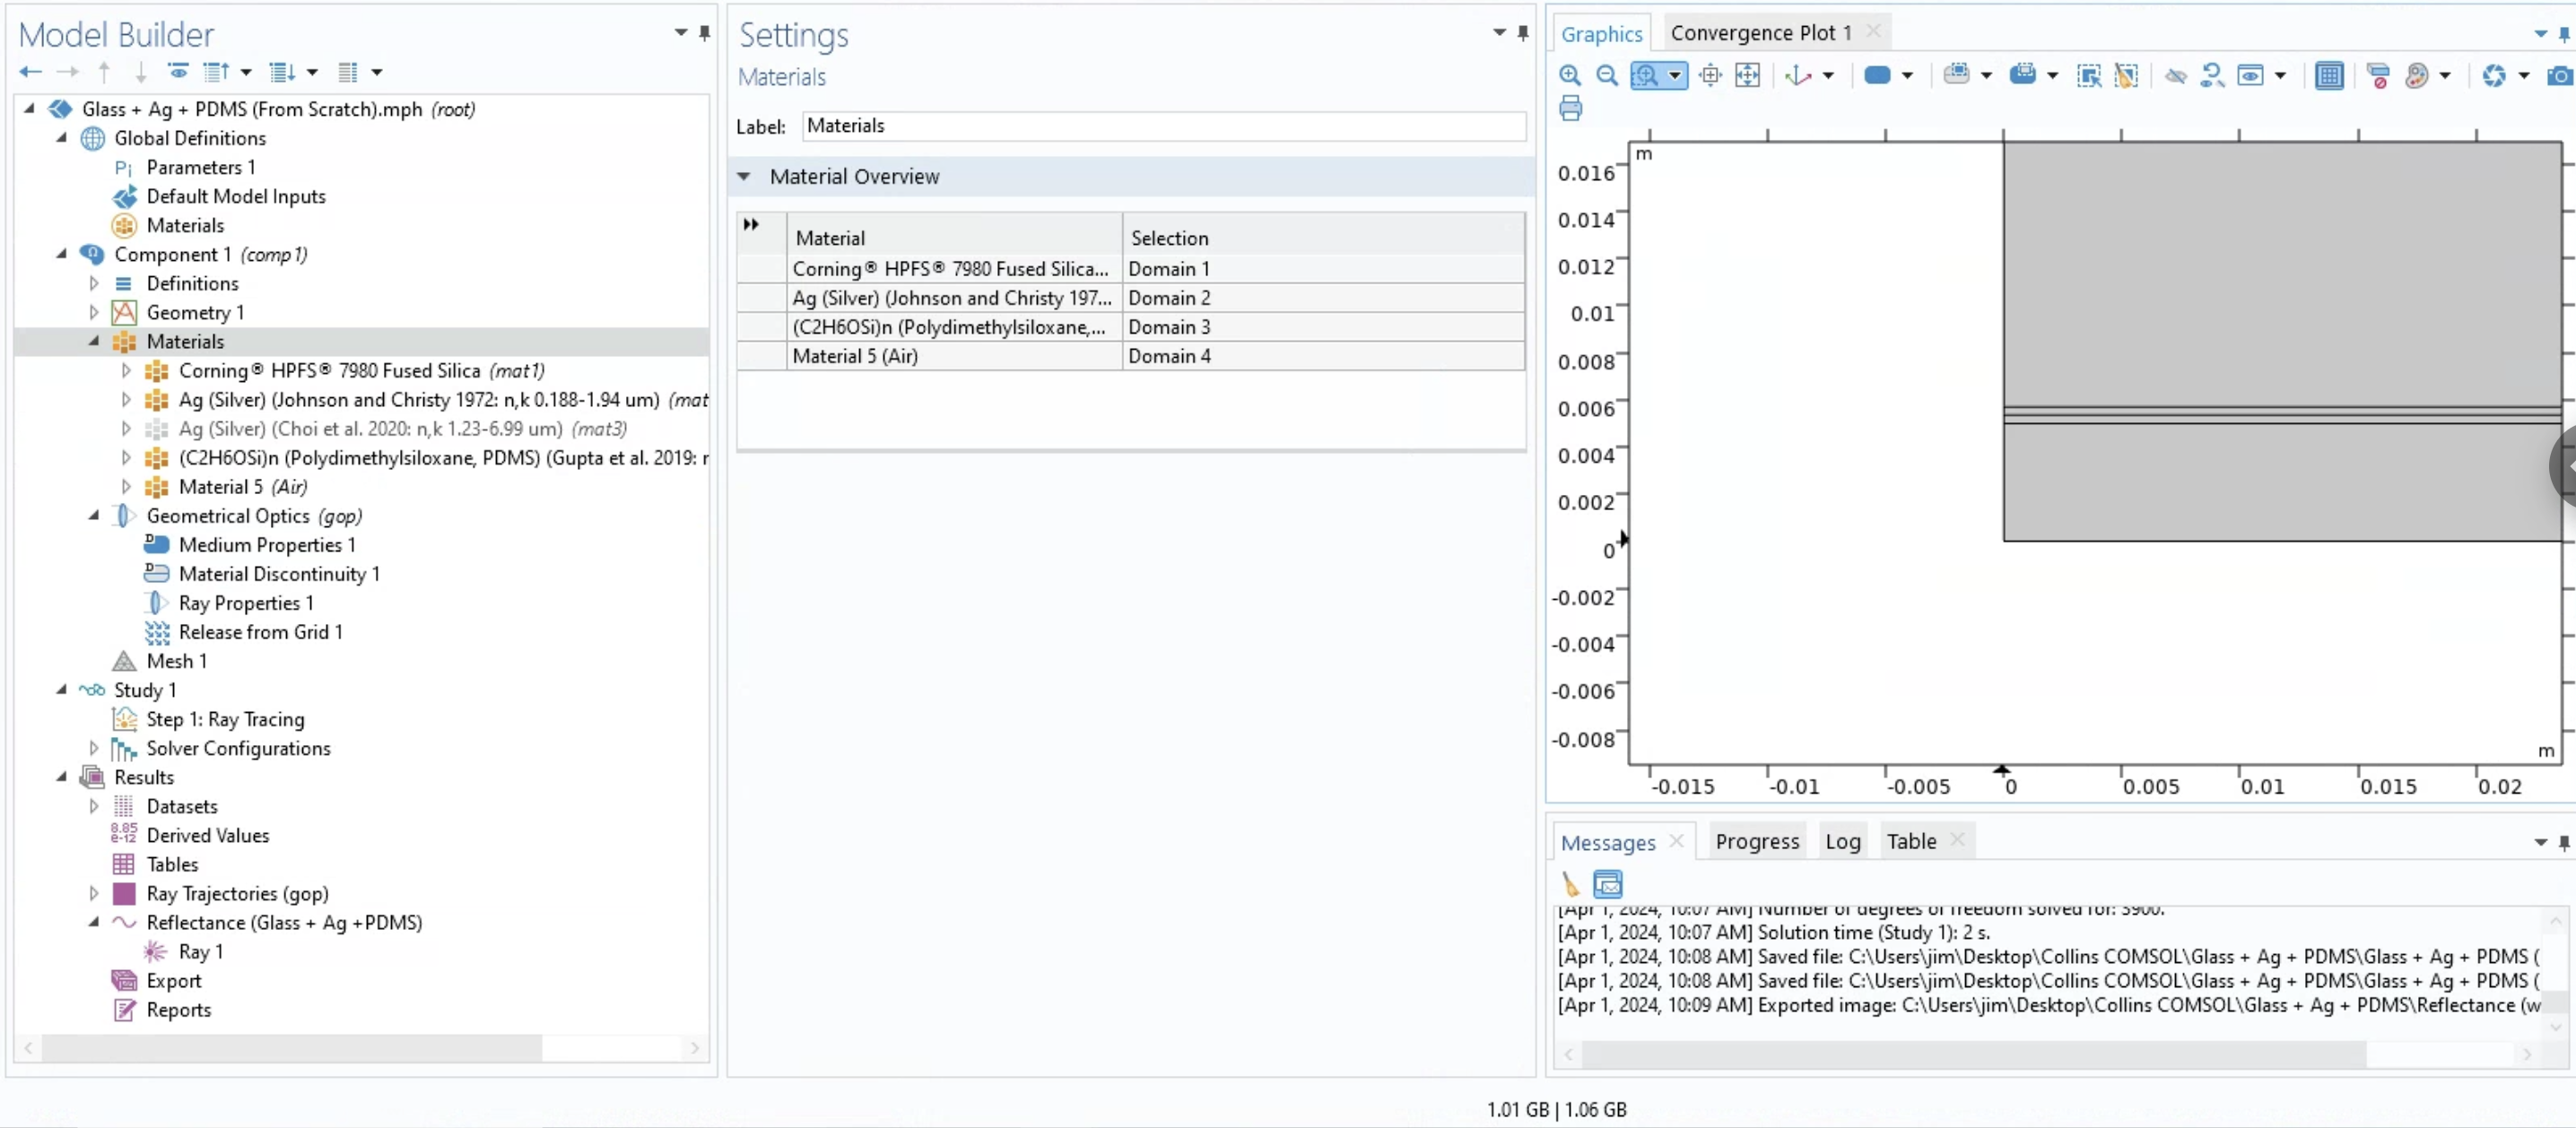
\includegraphics[width=0.7\textwidth]{Chapters/Figures/Chapter 4 Figures/COMSOL Desktop Layout for PDRC Analysis.png}
  \caption{COMSOL desktop setup for PDRC analysis demonstrating the simulation framework.}
  \label{fig:COMSOL-desktop-PDRC-setup}
\end{figure}

For simulations that span across various wavelengths, it is crucial to include the wavelength-dependence of the refractive indices of our materials. COMSOL tabulates $n(\lambda)$ for specific $\lambda$ measured in the literature. Then it interpolates between these experimentally measured points. This method allows for dynamic adjustment of a material's refractive index in response to changes in wavelength during simulations, providing a more accurate representation of the material's optical behavior.

\begin{figure}[H]
  \centering
  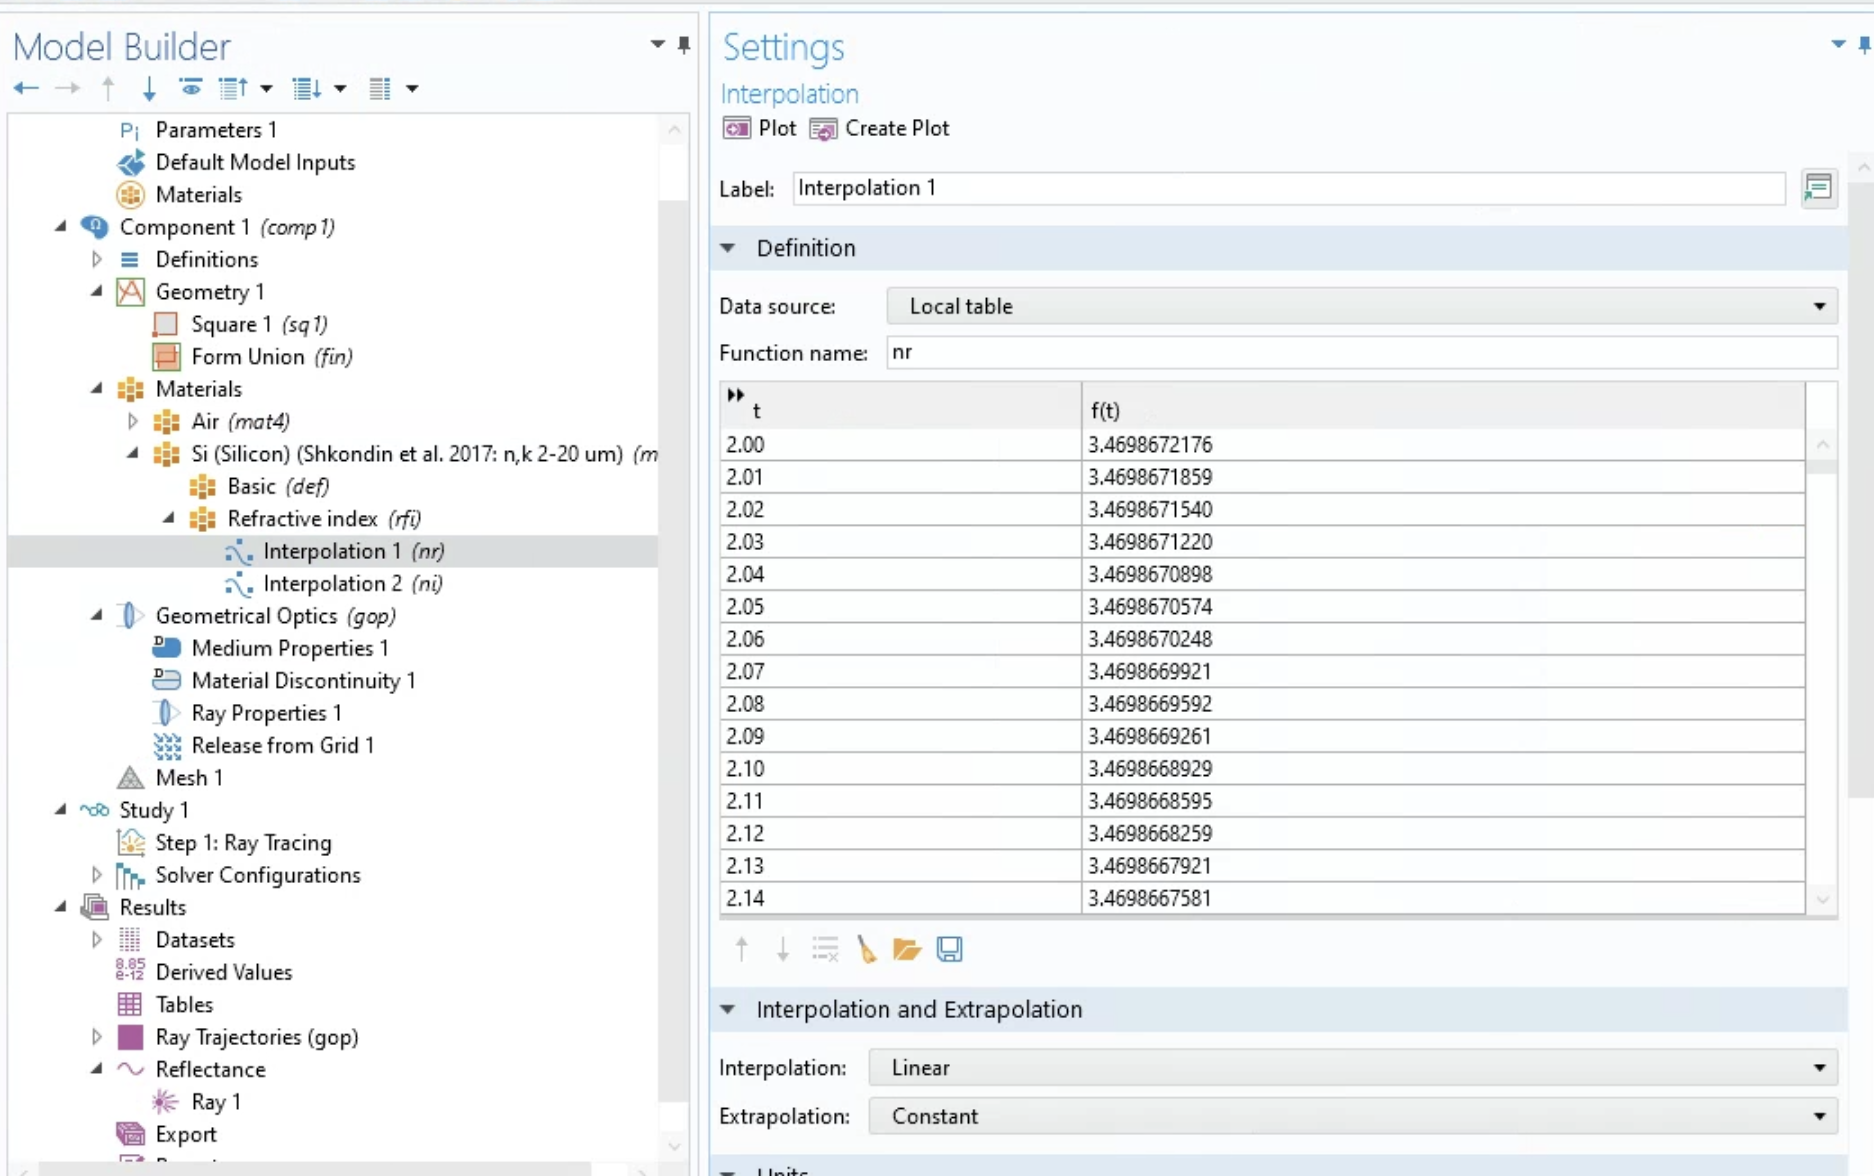
\includegraphics[width=0.7\textwidth]{Chapters/Figures/Chapter 4 Figures/Interpolation Table for the Silicon Substrate.png}
  \caption{Interpolation table for the silicon substrate, showing the wavelength-dependent refractive index.}
  \label{fig:interpolation-table-silicon}
\end{figure}

Utilizing the interpolation table enables the plotting of an interpolation function, offering a graphical representation of how refractive indices fluctuate with wavelength. This capability enriches the COMSOL simulation by providing a more precise depiction of light-material interaction over diverse wavelengths, a critical aspect in optics where dispersive phenomena play an important role.

% TODO: Add the interpolation plot for the silicon substrate
% \begin{figure}[H]
%   \centering
%   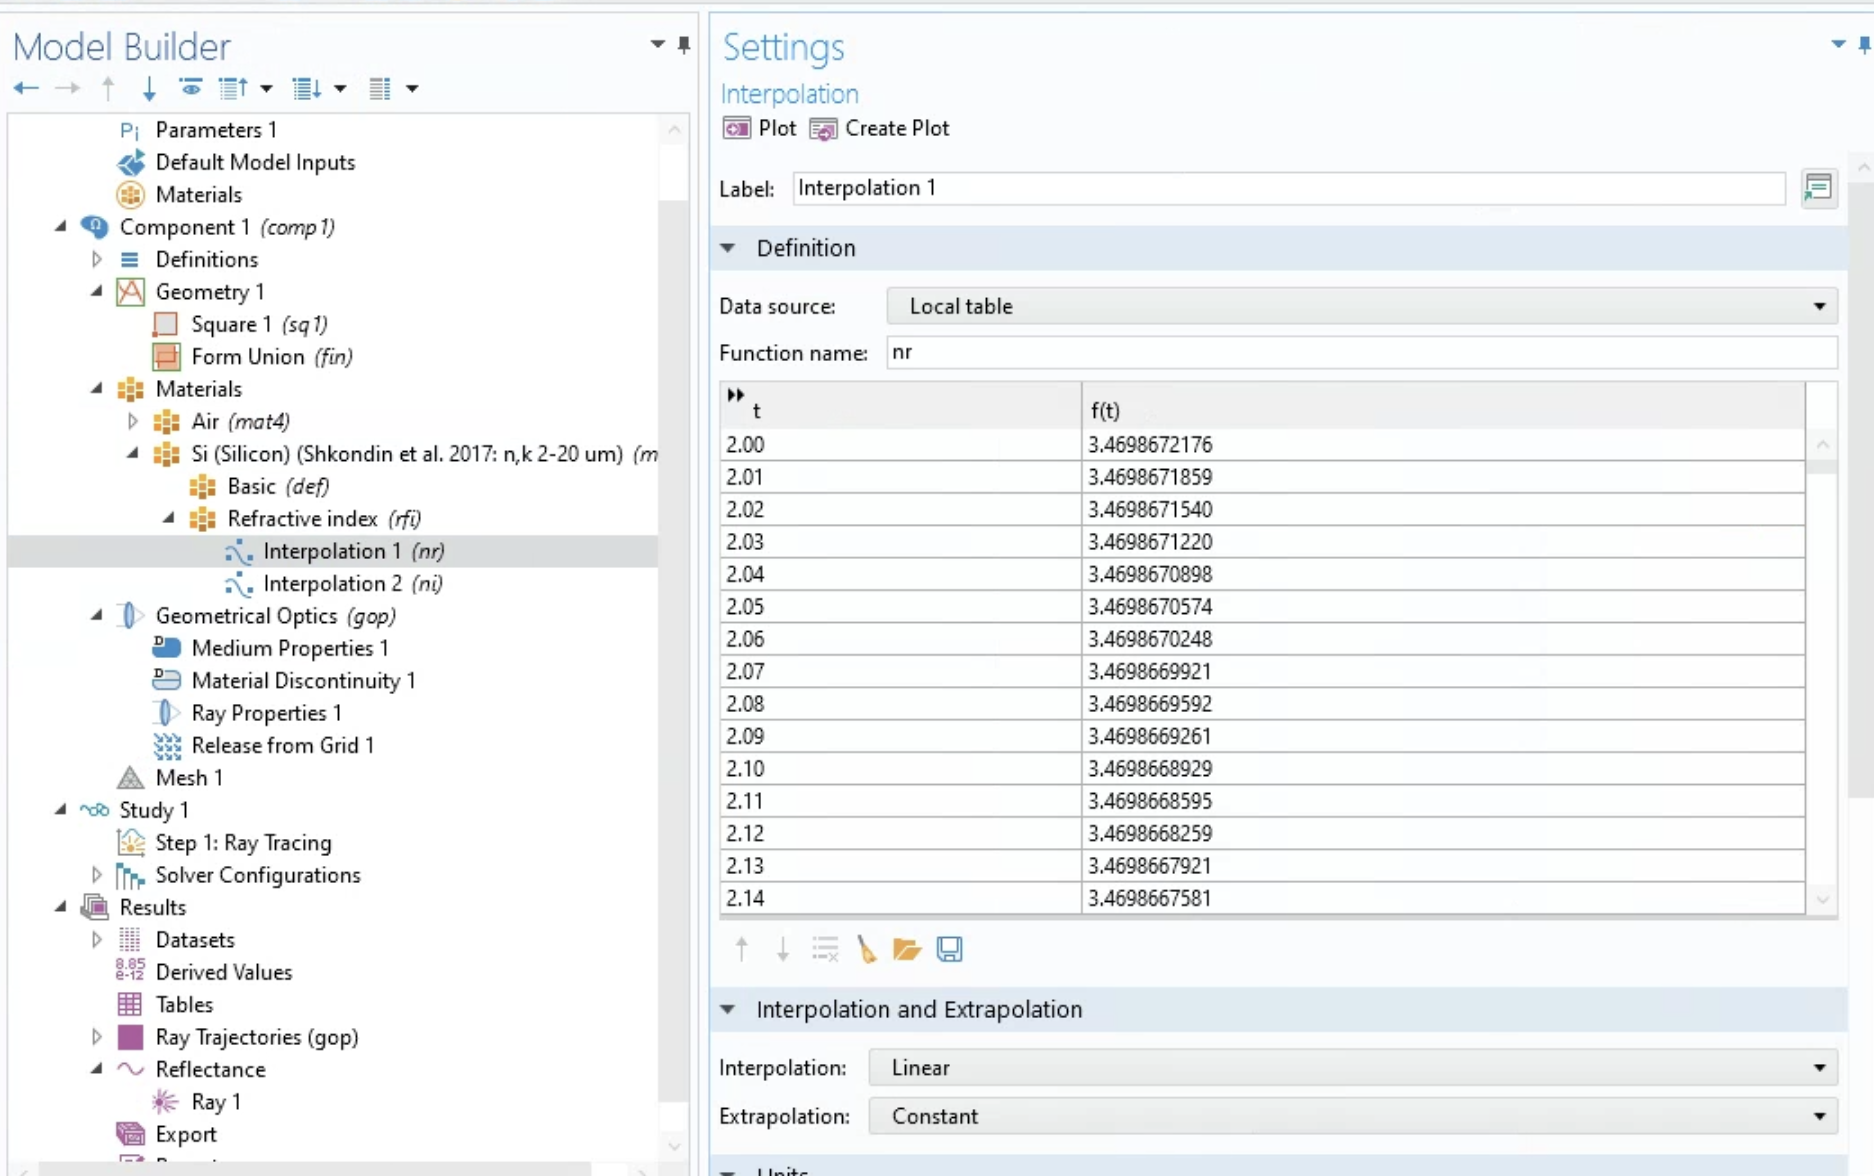
\includegraphics[width=0.7\textwidth]{Chapters/Figures/Chapter 4 Figures/Interpolation Table for the Silicon Substrate.png}
%   \caption{Interpolation table for the silicon substrate, showing the wavelength-dependent refractive index.}
%   \label{fig:interpolation-table-silicon}
% \end{figure}

For this reason, I selected Corning\texttrademark \space HPFS\texttrademark \space 7980 Fused Silica for the substrate, taking advantage of its accompanying interpolation function. It's vital to acknowledge that interpolation functions, which depict the wavelength-dependent refractive index variations of materials, can also be derived from experimental data found in scientific literature.

When generating a reflectance versus wavelength graph using only the glass substrate (specifically, Corning\texttrademark \space HPFS\texttrademark \space 7980 Fused Silica in this case), the reflectance indeed shows variation across different wavelengths.

\begin{figure}[H]
  \centering
  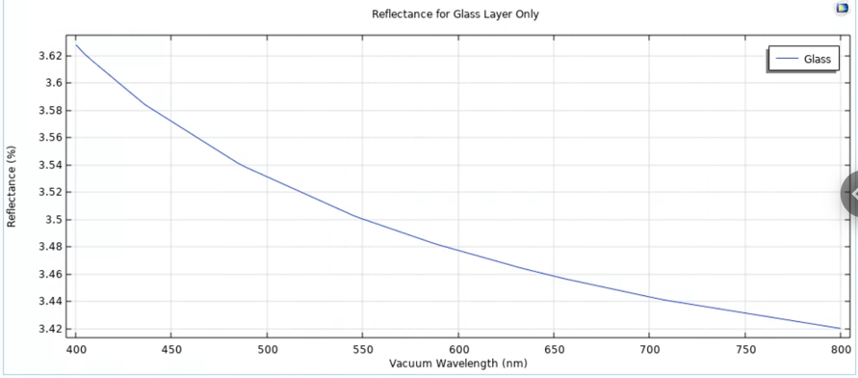
\includegraphics[width=0.7\textwidth]{Chapters/Figures/Chapter 4 Figures/Reflectance (Just Glass).png}
  \caption{Reflectance variation with wavelength for Corning\texttrademark \space HPFS\texttrademark \space 7980 Fused Silica.}
  \label{fig:Reflectance-variation-glass}
\end{figure}

Within the displayed wavelength range of $400 - 800$ nm, a sole substrate yields a reflectance below 4\%, which falls short of the desired high reflectivity within the solar spectrum for optimal PDRC performance. This observation underscores the need for integrating materials capable of meeting the dual objectives of high solar reflectance and substantial emissivity within the atmospheric window.

Focusing initially on enhancing solar reflectance, designs at Hudgings Lab incorporate silver on top the substrate due to its exceptional reflectivity in the solar spectrum. Having illustrated the outcomes with merely the glass substrate and underscored the importance of a highly reflective layer in the solar spectrum, I will venture into simulating the combined effects of glass and silver layers.

\subsection{Analysis of Silicon plus Silver Layers}
Next, I added a silver layer on top the glass substrate, recognizing the continued necessity for an interpolation function to accurately represent silver's refractive index across various wavelengths.

COMSOL offers a comprehensive collection of silver materials, each accompanied by interpolation tables that chart the refractive indices over preferred wavelength spans. The entry \emph{Ag (Silver) (Choi et al. 2020: n,k 1.23-6.99 um)} provides data on silver’s refractive indices from 1.23 to 6.99 ($\mu$m), where $n$ is the real component of the complex refractive index and $k$—the extinction coefficient—is the imaginary part, indicating the material's degree of light absorption.

\begin{figure}[H]
  \centering
  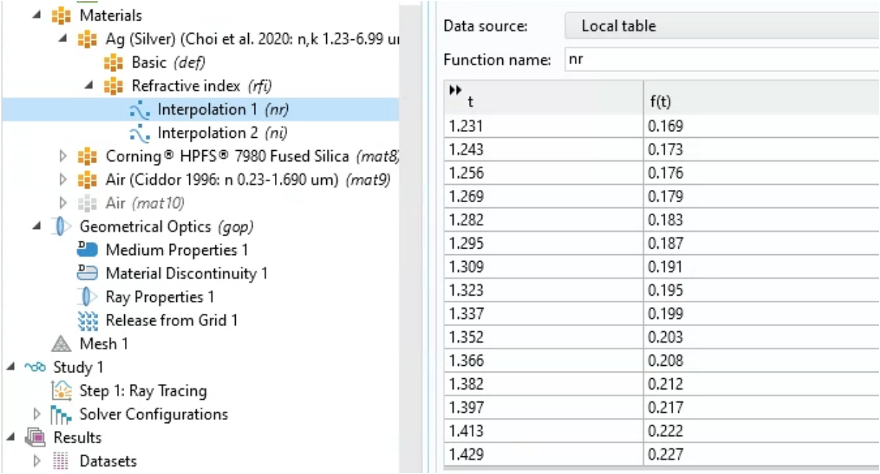
\includegraphics[width=0.7\textwidth]{Chapters/Figures/Chapter 4 Figures/Interpolation Table for Silver.png}
  \caption{Interpolation table for silver's refractive index.}
  \label{fig:Interpolation table for silver's refractive index}
\end{figure}

COMSOL's materials library offers various definitions of silver to cater to different wavelength ranges. For example, the definition \emph{Ag (Silver) (Johnson and Christy 1972: n,k 0.188-1.94 um)} provides an interpolation table covering 0.188-1.94 ($\mu$m).

The figures below display the outcomes utilizing \emph{Ag (Silver) (Johnson and Christy 1972: n,k 0.188-1.94 um)} and using \emph{Ag (Silver) (Choi et al. 2020: n,k 1.23-6.99 um)}, respectively.

\begin{figure}[H]
  \centering
  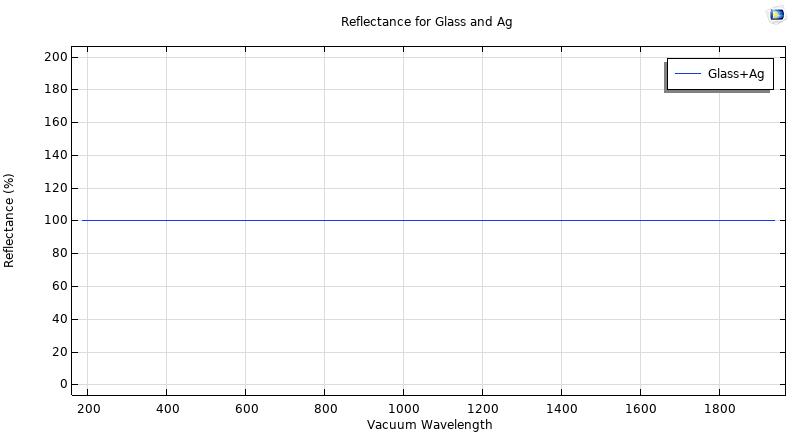
\includegraphics[width=0.7\textwidth]{Chapters/Figures/Chapter 4 Figures/Reflectance for glass and Ag (Johnson and Christy).png}
  \caption{Reflectance analysis for glass with Ag (Johnson and Christy).}
  \label{fig:Reflectance analysis for glass with Ag (Johnson and Christy)}
\end{figure}

\begin{figure}[H]
  \centering
  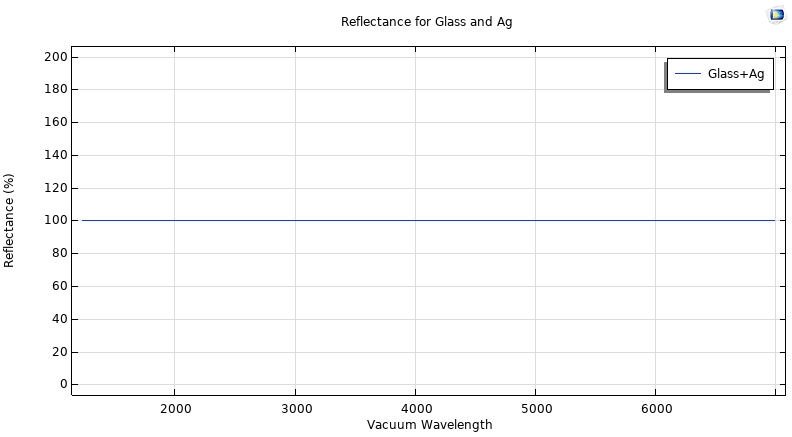
\includegraphics[width=0.7\textwidth]{Chapters/Figures/Chapter 4 Figures/Reflectance for glass and Ag for Choi et al.png}
  \caption{Reflectance analysis for glass with Ag (Choi et al.).}
  \label{fig:Reflectance analysis for glass with Ag (Choi et al)}
\end{figure}

These graphs mostly reflect the expected outcomes. Given silver's high reflectivity across the visible wavelength spectrum, we observe near 100\% reflectance within the visible range (400 - 700 nm).

\subsection{Analysis of Glass plus Silver plus PDMS Layers.}
In the final step, a PDMS layer was applied on top of the silver layer. This step also utilized a PDMS material equipped with a pre-defined interpolation function for its refractive index, specifically \emph{(C2H6OSi)n (Polydimethylsiloxane, PDMS) (Gupta et al. 2019: n 0.30-1.69 um)}.

\begin{figure}[H]
  \centering
  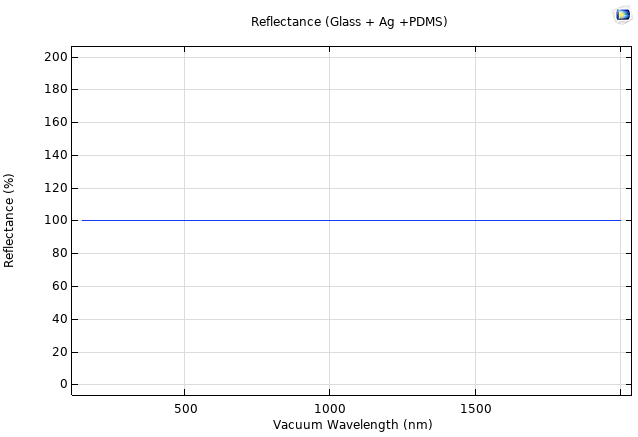
\includegraphics[width=0.7\textwidth]{Chapters/Figures/Chapter 4 Figures/Reflectance Results (Glass + Ag + PDMS).png}
  \caption{Reflectance analysis for a composite of glass, silver, and PDMS.}
  \label{fig:Reflectance analysis for glass, silver, and PDMS}
\end{figure}

This configuration resulted in reflectance maintaining a peak at 100\% across an extensive range of wavelengths.


---


We conclude our examination of optical phenomena using COMSOL. This chapter had two aims: first, to validate theoretical concepts like anti-reflectivity and high reflectance using COMSOL, and second, to initiate the simulation of basic PDRC configurations as designed at Hudgings Lab.

We began by evaluating anti-reflective strategies, ranging from simple to complex multilayer systems, against theoretical predictions from \emph{Introduction to Optics} by Frank L. Pedrotti et al. This comparison affirmed the accuracy of our simulations. Additionally, we modeled PDRC devices by layering glass, silver, and Polydimethylsiloxane (PDMS), revealing key optical properties essential for passive cooling effectiveness.

This chapter demonstrates the synergy between theoretical physics and computational modeling, offering a solid foundation for future research to expand upon. It underscores the importance of simulation in confirming theoretical models and opens avenues for improving PDRC device design.

Looking forward, the results from this chapter not only validate our understanding of optical principles but also suggest strategies for enhancing PDRC performance through material and design optimization.